%%%%%%%%%%%%%
\section{Aplication to Synthetic Data}

%%%
\subsection{Simple Simulation: Validating the Methodology}

\noindent{We applied the proposed method in a numerical simulation of a geological thin-section of dimensions 1000 μm x 1000 μm in a regular grid (1000 x 1000) for estimating the magnetization directions of four spherical sources uniformly magnetized (but with different directions), according to \cref{tab:ModelTab}. Totaling an observation number N = $10^6$ obtained at a sensor-sample distance of 5 μm and a grid spacing of 1 μm. Subsequently, the data vector was contaminated with a pseudo-random noise of normal Gaussian distribution with a zero mean and 25 nT standard deviation, as shown in \cref{fig:SimpleSynthetic}a.}

\bigskip

\floatsetup[table]{capposition=top} % to put the caption on the top of the table
% If you use beamer only pass "xcolor=table" option, i.e. \documentclass[xcolor=table]{beamer}

\begin{table}[htbp]
\caption{Initial position and magnetization parameters for each spherical source.}
\label{tab:ModelTab}
\resizebox{1.0\textwidth}{!}{
\tiny
\begin{tabular}{ccccccc}
\hline   
\rowcolor[HTML]{FFFFFF} 
\cellcolor[HTML]{FFFFFF}                         & \multicolumn{3}{c}{\cellcolor[HTML]{FFFFFF}Center coordinates}                    & \multicolumn{3}{c}{\cellcolor[HTML]{FFFFFF}Magnetization}     \\
\rowcolor[HTML]{FFFFFF} 
\multirow{-2}{*}{\cellcolor[HTML]{FFFFFF}Sphere} & Xc ($\mu m$) & Yc ($\mu m$) & Zc ($\mu m$) & m ($A \cdot m^2$) & D (\textdegree) & I (\textdegree) \\  \hline   
1                                                & 250.00                       & 250.00                       & 5.30                       & 8.70e-15               & -140.00                        & -30.00                 \\
\rowcolor[HTML]{FFFFFF} 
2                                                & 500.00                       & 500.00                       & 7.75                       & 7.63e-15               & -70.00                        & -50.00                 \\
3                                                & 750.00                       & 750.00                       & 8.50                       & 6.21e-15               & 10.00                        & 62.00                 \\
\rowcolor[HTML]{FFFFFF} 
4                                                & 200.00                       & 800.00                       & 10.00                       & 4.97e-15               & 125.00                        & 22.00                  \\ \hline                 
\end{tabular}
}
\end{table}



\bigskip

\noindent{The first step is to apply the upward continuaton filter, which transforms the potencial field measured on a surface into one measured at a higher surface level \citep{Blakely1996}, therefore smoothing out high frequency noise. This first step is always needed in high frequency noisy data, since the Euler equation requires the first derivatives of potencial field. If this step is negleted or badly elaborated, the high frequency noise propagation during the application of the derivative filters will cause future errors in the next methodological stage.} 

\noindent{The next step is to calculate the magnetic total gradient (or horizontal gradient) filter in order to highlight the anomaly signal of each source within its own boundaries, then we apply the blob detection algorithm \citep{VanderWalt2014} to obtain a robust positioning of each source data window (\cref{fig:SimpleSynthetic}b).}

\begin{figure}[htbp]
\centering
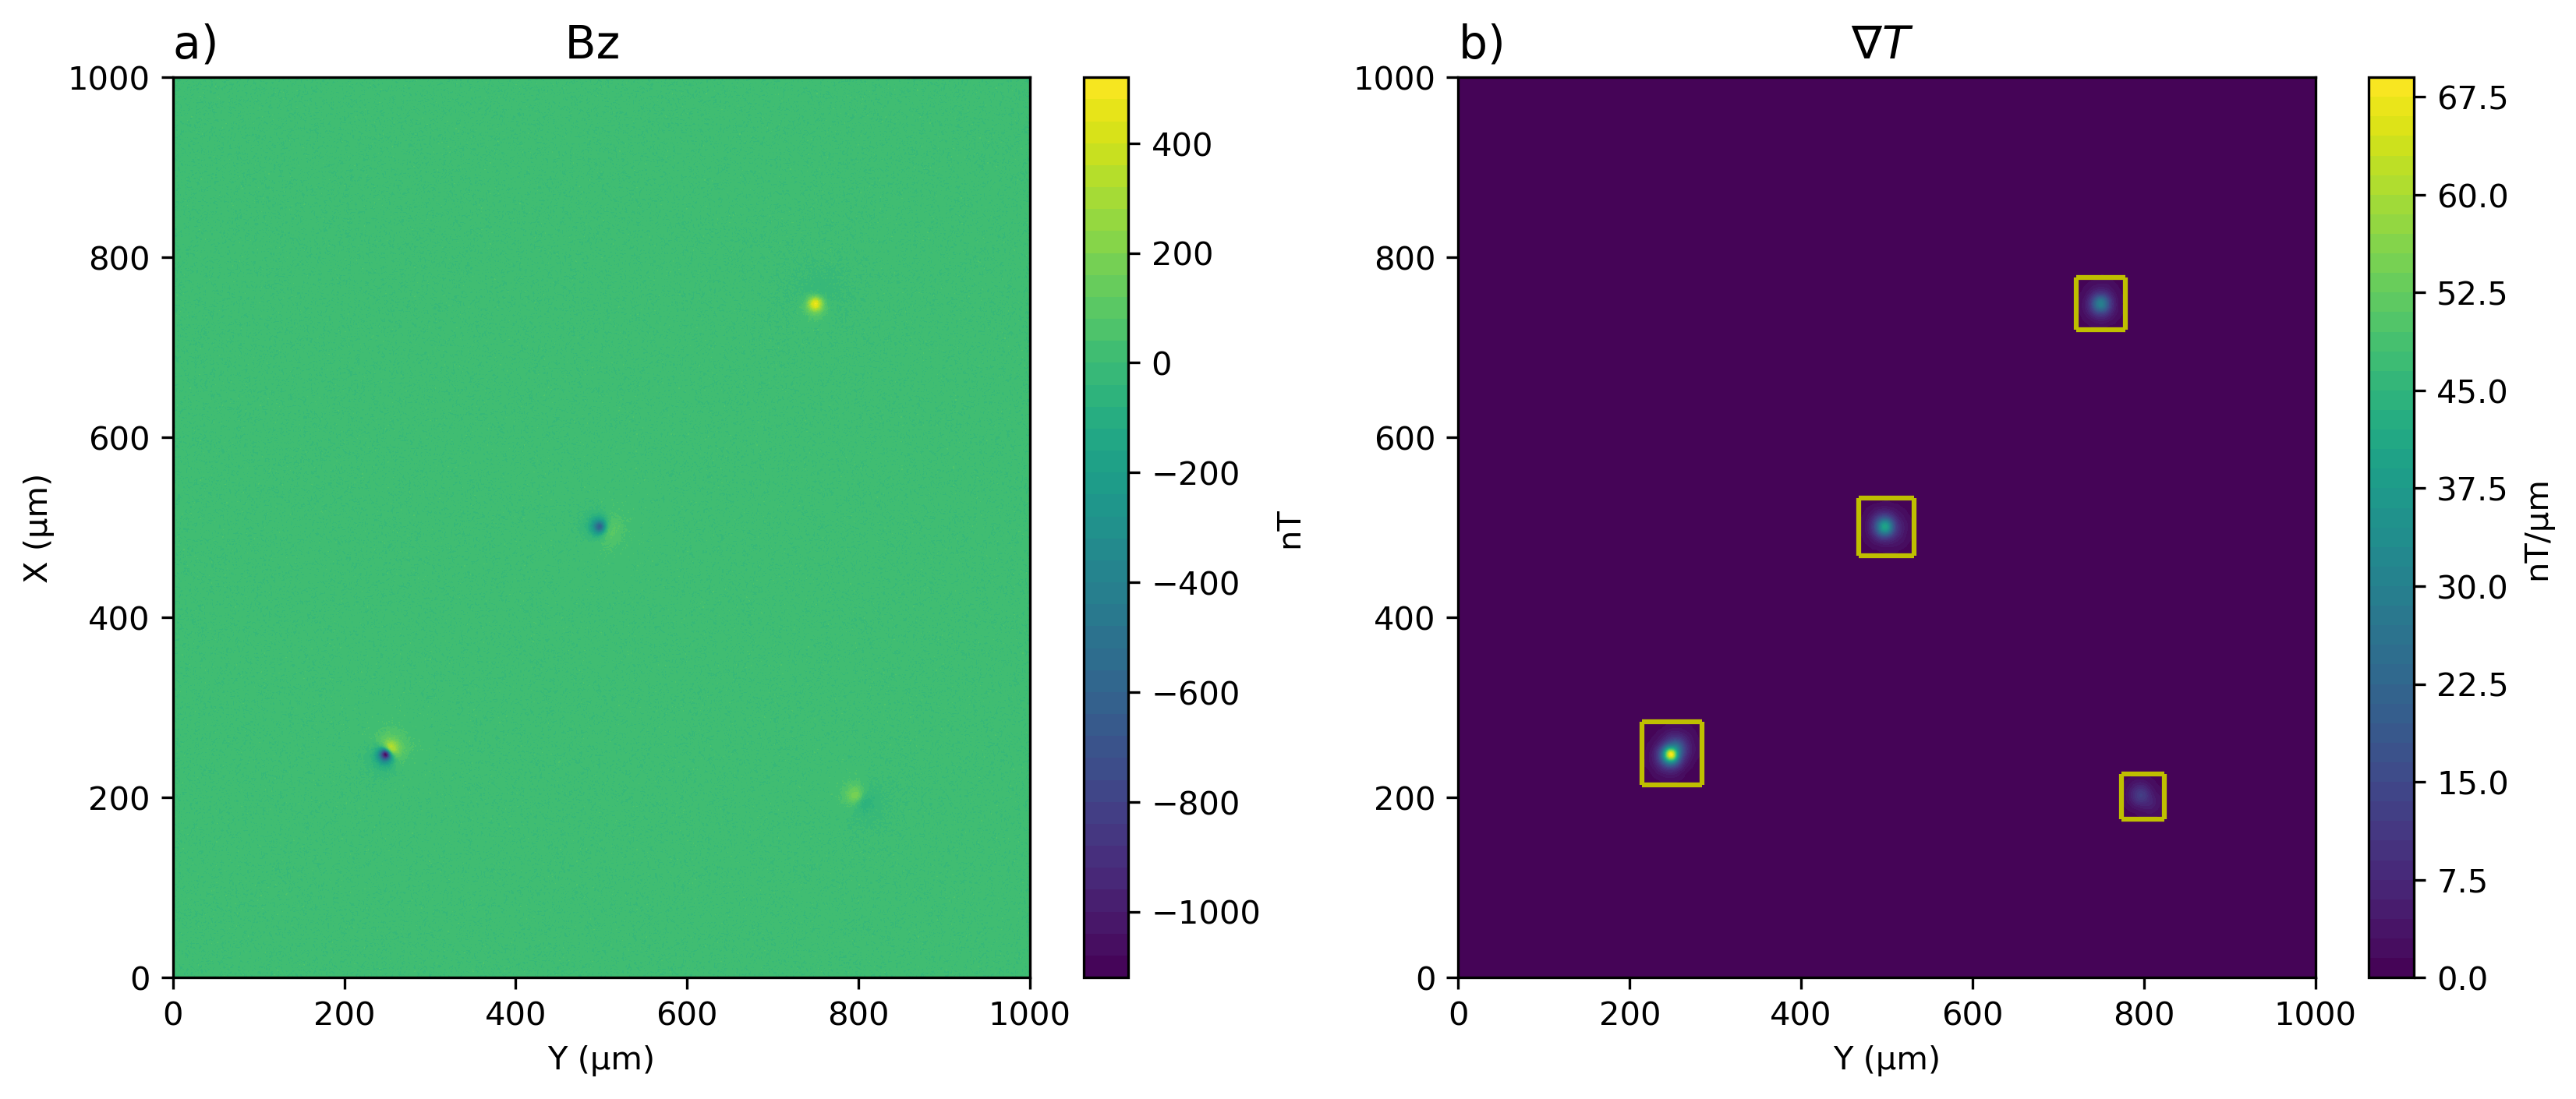
\includegraphics[width=1.0\textwidth]{SimpleSynthetic.png}
\caption{a) Synthetic data contaminated with psedo-random normal noise. b) Individual sources window position (yellow squares) obtained with the blob detection algorithm applied on the total gradient map.}
\label{fig:SimpleSynthetic}
\end{figure}

\bigskip

\noindent{After isolante the potencial field data and first derivatives for each source, we can solve the 3D Euler deconvolution \cref{eq:euler2} proposed by  \cite{Reid1990}, one for each subarea selected (window data), by assuming the structural index of a sphere/punctual source (N = 3). Thus, obtaining a sturdy result for the central positioning (Xc, Yc, Zc) of each source causing the magnetic potential anomaly in the observed data set, as shown in \cref{tab:InversionTab}.}

\noindent{The last step consists of using the central positions of each source, obtained with Euler's method, as an input parameter for inverting the original noisy data (\cref{fig:SimpleSynthetic}a) to find the least squares (or robust) approximation solution for the vector of cartesian magnetic moments ($\bar{m}$). With this, the magnetization directions (D and I) and the intensity of the magnetic moment can be estimated using equations (\cref{eq:sphere16,eq:sphere17,eq:sphere17_m}), as well as the uncertainty propagation of this inversion, using equations (\cref{eq:sphere21,eq:sphere22,eq:sphere22_m}) and considering $\sigma$ = 25nT. The results obtained with the least squares estimator can also be seen in \cref{tab:InversionTab}.}

\bigskip

% If you use beamer only pass "xcolor=table" option, i.e. \documentclass[xcolor=table]{beamer}

\begin{table}[htbp]
\caption{Positioning and magnetization parameters recovered with the inversion.}
\label{tab:InversionTab}
\resizebox{1.0\textwidth}{!}{
\begin{tabular}{ccccccc}
\hline   
\rowcolor[HTML]{FFFFFF} 
\cellcolor[HTML]{FFFFFF}                         & \multicolumn{3}{c}{\cellcolor[HTML]{FFFFFF}Center coordinates}                    & \multicolumn{3}{c}{\cellcolor[HTML]{FFFFFF}Magnetization}     \\
\rowcolor[HTML]{FFFFFF} 
\multirow{-2}{*}{\cellcolor[HTML]{FFFFFF}Sphere} & Xc ($\mu m$) & Yc ($\mu m$) & Zc ($\mu m$) & m ($A \cdot m^2$) & D (\textdegree) & I (\textdegree) \\  \hline   
1                                                & 250.28           & 250.19           & 5.38           & 8.82e-15  $\pm$  1.39e-17           & -140.22  $\pm$  0.11           & -30.04  $\pm$  0.08           \\
\rowcolor[HTML]{FFFFFF} 
2                                                & 500.46           & 500.50           & 7.77           & 7.67e-15  $\pm$  1.90e-17           & -69.42  $\pm$  0.26           & -49.85  $\pm$  0.15           \\
3                                                & 750.73           & 750.72           & 8.57           & 6.31e-15  $\pm$  1.99e-17           & 9.06  $\pm$  0.50           & 62.34  $\pm$  0.22           \\
\rowcolor[HTML]{FFFFFF} 
4                                                & 200.30           & 800.92           & 10.00           & 4.94e-15  $\pm$  3.01e-17           & 124.63  $\pm$  0.39           & 21.76  $\pm$  0.27           \\ \hline                 
\end{tabular}
}
\end{table}



\noindent{It is important to emphasize that \cite{OliveiraJr.2015} proved that the magnetization directions (D and I) recovered by the least squares estimator is sensitive to variations in the horizontal coordinates (x and y) of the magnetic sources central positions. While, the same being practically insensitive to variations in depths. Thus, the same authors consider Euler deconvolution method as an adequate technique to estimate the central positions that will be used as a priori information for inversion. This occurs mainly because, when well performed, the recovery of the horizontal coordinates of sources central position is considerably accurate, while the vertical coordinate can undergo greater variation \citep{Silva2003, Melo2013}, even so the inversion will still provide extremely satisfactory results. The high sensitivity of Euler deconvolution to high frequency noise can also be easily overcome with the proper application of the upward continuation filter.}



\subsection{Complex Simulation: Testing Applicability}

